\subsection{Capsicum}
\label{subsec:capsicum}
%<Kritika>

Capsicum is one user space implementation for a capability based access control system developed at the University of Cambridge Computer Laboratory. \footnote{https://www.cl.cam.ac.uk/research/security/capsicum/} It is a lightweight framework that extends the POSIX API. It implements capabilities by modifying current kernel primitives as well as by performing sandboxing techniques in the userspace. It provides capabilities for logical applications by implementing \textit{compartmentalization} of the application. The first implementation for Capsicum was on FreeBSD 8.x, and as a result of more research being conducted, it is now being released along with FreeBSD 9.0 as an experimental feature.

The implementation of capabilities by extending, rather than gives the applications the benefit of having least-privilege operations in the system. Separation or compartmentalization is a popular technique used by OSs today to help security-critical applications in dealing with vulnerabilities. It limits the impact of the system by exposing only a small part or compartment of the entire system to the vulnerability.The other critical aspect of implementing such a system is to make sure that this is achieved by minimum effort.

Capsicum achieves this by implementing certain security primitives like \textit{capability mode} and \textit{capabilities.} Some of the implementation modifies the kernel level primitives, while others are for userspace implementation. These primitives together support logical compartmentalization of the application. Once the application code is separated into individual logical parts, we can run independent sandboxes to form logical applications as shown in Figure \ref{compartment}.

\begin{figure}[h]
\centering
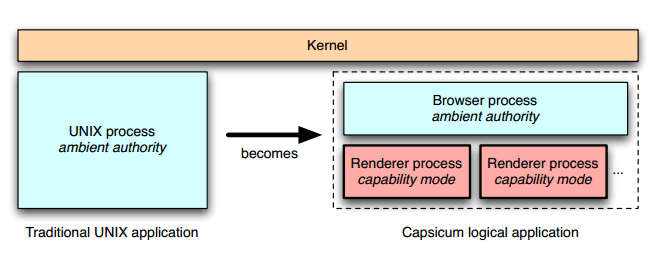
\includegraphics[scale=0.45]{img/capcisum_sandbox}
\caption{Logical compartmentalization of applications}
\label{compartment}
\end{figure}

Following is the list of all such primitives:

		\begin{itemize}
		    \item \textbf{capabilities:} file descriptors with refined privileges.
   		    \item \textbf{capability mode:} implementing sandboxing so as to deny access to global namespaces.
    		    \item \textbf{process descriptors:} replacing capability-centric process IDs. 
    		    \item \textbf{anonymous shared memory objects:} an extension to the POSIX shared memory API.
    		    \item \textbf{rtld-elf-cap:} constructing sandboxed applications from run-time linkers by modifying ELF 
    		    \item \textbf{libcapsicum:} library to create and use capabilities components
    		    \item \textbf{libuserangel:} library allowing sandboxed applications or components to interact with user angels, such as Power Boxes.
    		    \item \textbf{chromium-capsicum:} Google's Chromium web browser that provides effective sandboxing of high-risk web page rendering.

		\end{itemize}
		
Capsicum has a host of capability implementation that can be used, but they leave the end user to use his/her discretion in order to maximize the security impact for their respective application. Implementing the \textit{capability mode} for example, implies that a process flag is set by the system call. Once this flag is set, the system goes into the capability mode, and the process is then denied access to global namespaces. In addition to this, in the capability mode, the access to the certain system calls is also limited.

In Capsicum, capabilities can also be implemented using file descriptors. File descriptors have certain properties that are considered desirable in a capability system, like being a tokens of authority, being unforgeable as well as being able to pass the properties through inheritance. In Capsicum, the \textit{cap\_new} system call extends the file descriptor by creating a new capability and a set of rights. These rights get checked by \textit{fget} which performs the conversion of file descriptor  arguments to system calls to in-kernel references.